% !TEX encoding = UTF-8
% !TEX TS-program = pdflatex
% !TEX root = ../tesi.tex

%**************************************************************
\chapter{Sperimentazione}
\label{cap:sperimentazione}
%**************************************************************
\section{Popolamento dei database}

Portata a termine la predisposizione di strumenti ed ambienti di lavoro, e determinata la struttura dei database, è ora possibile andare a caricare al loro interno i dati che li popolano.\\

\subsection{Creazione dei dati}
Per effettuare test di carico sui database è necessario che questi contengano una quantità di dati elevata. Si è scelto di generare dei dati ``fantoccio'' per automatizzare il processo.\\
Scegliendo lo strumento giusto, si possono così ottenere dati realistici in quanto a contenuto e dimensione, per fare in modo che le misurazioni effettuate sui tempi di esecuzione delle query abbiano un significato anche al di fuori dell'ambiente di test.\\
Sebbene inizialmente i dati siano stati generati tramite siti online che permettono di esportare fino a un migliaio di tuple, è presto diventato chiaro come questo avrebbe rallentato di molto il processo di popolamento, rendendolo anche più complesso.\\

\noindent Si è quindi deciso di ricorrere ad uno strumento diverso, disponibile come pacchetto di \textit{Node.js} e installabile tramite \gls{npm}\ped{G} (\textit{node package manager}) in modo da poter essere utilizzato da linea di comando.\\
Questo strumento, \textit{datamaker}, è in grado di generare un numero arbitrario di records basandosi su template forniti dall'utente. Senza contare che è molto più rapido dei sistemi online.\\
Grazie a \textit{datamaker} è stato possibile generare dei dati fittizzi secondo specifiche personalizzate, in quantità elevate.\\
Questo sistema garantisce anche un buon grado di consistenza, poiché rimane la traccia dello schema utilizzato in forma di template, cosa che invece andava spesso persa nei processi online. Anche grazie a questo è stato possibile generare dati affidabili su cui condurre i test, variando la quantità di dati presente in un file di import senza alterare in alcun modo lo schema che definisce come questi dati vengono costruiti.\\


\subsection{Formato dei dati}
Quando si parla di formato dei dati è bene specificare la differenza tra formato di importazione dei dati e formato dei dati all'interno dei database.\\
MongoDB salva i propri dati in formato \texttt{BSON}, una versione estesa del più comune \texttt{JSON}. Per la costruzione di tali dati è sufficiente creare dei file in formato \texttt{JSON}, e il database si occupa del resto.\\
Utilizzando l'interfaccia di Compass è tuttavia possibile importare i propri dati da un file in formato \texttt{CSV}. Questo può facilitare il processo, specialmente quando si è più abituati a lavorare con questo tipo di formato.\\
Per quanto riguarda PostgreSQL, anche l'interfaccia di pgAdmin permette di importare i propri dati da file, che devono essere in formato \texttt{CSV}.\\
Tale file verrà elaborato e il suo contenuto trasferito automaticamente nelle tabelle su cui si esegue questa operazione.\\

\noindent Nel caso di questo progetto, si è scelto di utilizzare file in formato \texttt{CSV} per l'importazione all'interno del database relazionale e file in formato \texttt{JSON} per l'importazione nel database NoSQL.\\
Nonostante il contenuto di documenti e tabelle sia pressochè lo stesso, proprio perchè il confronto abbia senso, la differenza sta proprio nella struttura in cui sono organizzati questi dati. Per questo motivo non sarebbe stato possibile usare lo stesso file \texttt{CSV} per popolare entrambi i database, nonostante gli strumenti utilizzati lo avrebbero permesso.\\

%**************************************************************
\section{Metodi di monitoraggio dei risultati e creazione delle query}
Per confrontare le performance delle query nei due database è necessario raccogliere dei dati sulla loro esecuzione. Nello specifico, serve sapere quanto tempo impiegano le query per essere eseguite.\\
Il tempo impiegato, tuttavia, può essere fuorviante. La notifica che per esempio riceviamo nel software pgAdmin si riferisce al tempo totale di elaborazione della richiesta, che per esempio comprende anche la latenza di connessione al network, e altri dati non relativi al tempo strettamente necessario all'esecuzione della query.\\

Per eseguire un confronto più preciso è necessario capire come estrapolare i dati che cerchiamo in entrambe le basi di dati.

\subsection{Estrapolare i tempi di esecuzione in PostgreSQL usando pgAdmin}
PostgreSQL, come molti database relazionali e non, mette a disposizione il metodo \texttt{EXPLAIN}. Quando questo viene utilizzato in testa ad una query, il risultato che si ottiene è una serie di informazioni riguardanti la sua esecuzione. Tra i vari parametri di questo metodo, quelli più interessanti per questo caso d'uso sono \texttt{ANALYZE} e \texttt{TIMING}, che possono essere specificati per ottenere informazioni specifiche riguardanti il tempo di esecuzione delle varie sezioni di query.\\
Le query che vengono eseguite in questo modo vengono comunque portate a termine dal database, anche se il risultato di eventuali operazioni di \texttt{SELECT} non viene mostrato a schermo.\\
Per impedire che questo accada è bene seguire la query con un'operazione di \textit{rollback}.\\

\noindent pgAdmin permette di utilizzare il metodo \texttt{EXPLAIN} eseguendo la query che si vuole analizzare in uno spazio apposito dell'interfaccia. Il risultato dell'operazione viene riportato in una tabella per semplificare la lettura, mentre vengono messi a disposizione anche una vista a grafo ed una tabella più complessa per il confronto tra tempi stimati dal metodo e tempi reali di esecuzione.\\
Agli scopi di questa tesi, verranno prese in considerazione le informazioni riportate nella tabella principale, dove i tempi di completamento delle operazioni sono all'occorrenza separati nei vari pezzi che compongono la query.

\subsection{Estrapolare i tempi di esecuzione in MongoDB usando Compass}
All'interno di MongoDB si utilizza un linguaggio specifico per estrapolare informazioni dai database. Se per i database relazionali si parla di Structured Query Language, in questo caso invece si usa \textit{MQL}, ovvero MongoDB Query Language, basato sulla sintassi di \textit{JavaScript}.\\

\noindent Attraverso un'ampia selezione di metodi questo linguaggio offre la possibilità di effettuare tutte le \gls{operazioni CRUD}\ped{G}, oltre ad alcune altre funzionalità che possono tornare utili in varie situazioni, dalla gestione dei database alla misurazione delle prestazioni delle query.\\
Utilizzando Compass, è poi possibile sfruttare una finestra apposita dell'interfaccia grafica per eseguire l'\textit{explain plan} di alcune query. Questa funzionalità è limitata tuttavia all'analisi del metodo \texttt{find()}, che corrisponde ad una select in \gls{SQL}\ped{G}.\\
Per gli altri metodi è necessario approfondire il funzionamento del linguaggio di MongoDB per effettuare manualmente una ricerca sui tempi di esecuzione delle varie operazioni.\\
Una volta determinato quali metodi concatenare per ottenere i risultati desiderati, è poi necessario eseguire tali comandi nella shell di MongoDB. Fortunatamente questa è accessibile sempre dall'interfaccia di Compass, rendendo il processo più lineare.\\


%**************************************************************
\section{Statistiche sulle query eseguite sui due database}
Il confronto tra i due database è stato effettuato creando sette copie di query volte ad ottenere lo stesso risultato sia sul database relazionale che su quello documentale. Il risultato di questo tipo di analisi evidenzia come le diverse strutture di archiviazione dei dati e le diverse architetture all'interno dei database possono garantire risultati migliori o peggiori in base ai casi d'uso.\\
La creazione delle query è stata basata su una esemplificazione dei casi d'uso più comuni individuati per InvoicheChannel.

\subsection{Query 1}
La prima query, esposta in Figura 6.1, è piuttosto semplice. Effettua una ricerca generica per elencare tutte le invoice e le operations ad esse collegate.\\

\begin{figure}[htbp]
\begin{center}
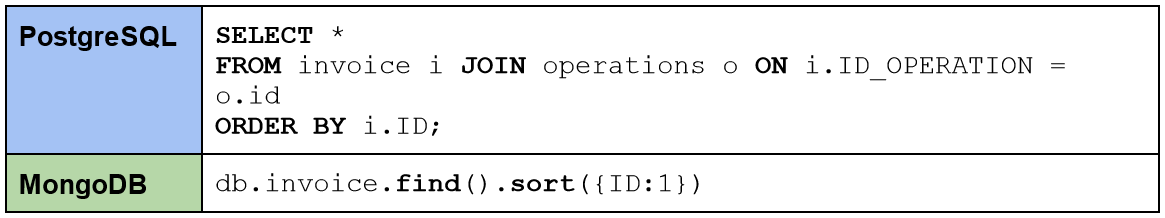
\includegraphics[height=7em]{immagini/query/query1.png}
\caption{Codice della query numero 1, scritto in entrambi i linguaggi}
\end{center}
\end{figure}

\noindent Facciamo notare che PostgreSQL crea automaticamente gli indici sulle primary keys, quindi sono stati indicizzati anche i campi ID dei documenti in MongoDB. Questo è stato fatto per effettuare un confronto alla pari, ma è anche dovuto al fatto che intorno ai 200.000 documenti MongoDB non permette più di effettuare operazioni di \texttt{sort()} se non viene integrato l'uso di indici.\\

\noindent Nel seguente grafico (Figura 6.2) possiamo vedere i risultati del confronto sui tempi ottenuti ripetendo la stessa query su database popolati con un numero sempre maggiore di elementi.\\

\begin{figure}[htbp]
\begin{center}
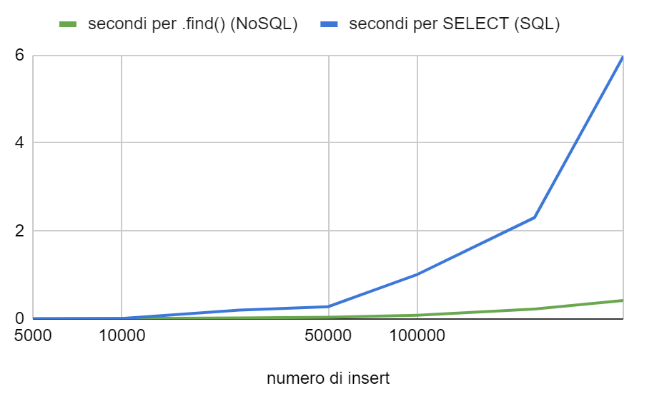
\includegraphics[height=20em]{immagini/query/query1_results.png}
\caption{Risultato del confronto, query numero 1}
\end{center}
\end{figure}

\noindent Dal grafico si evince quanto già scoperto durante lo studio delle tecnologie coinvolte nel confronto. L'utilizzo di documenti incorporati (in questo caso i dati dell'operation che riguarda l'invoice sono contenuti nel documento dell'invoice stessa) permette a MongoDB di evitare le operazioni di \texttt{join}, che rallentano di molto l'esecuzione delle query in PostgreSQL.\\

\noindent Possiamo notare come la differenza sia ancora più evidente se cerchiamo gli stessi dati applicando una condizione di ricerca.\\

%--------------------------------------------------------------

\subsection{Query 2}
Con la seconda query, esposta in Figura 6.3, cerchiamo tutte le invoice e le operations ad esse associate, questa volta limitandoci alle sole fatture che soddisfano una specifica condizione sul proprio numero identificativo.\\

\begin{figure}[htbp]
\begin{center}
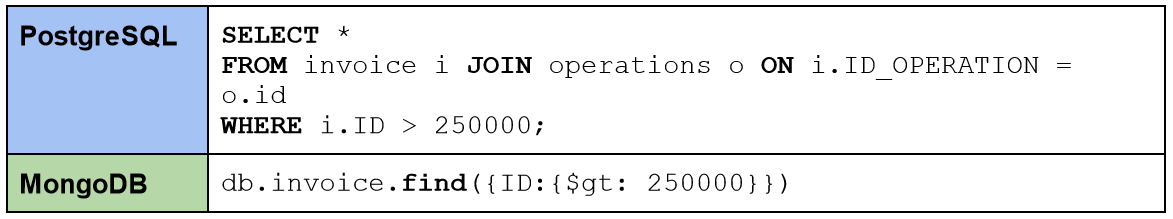
\includegraphics[height=7em]{immagini/query/query2.png}
\caption{Codice della query numero 2, scritto in entrambi i linguaggi}
\end{center}
\end{figure}

\noindent In questo caso PostgreSQL farà uso di indici per andare a scorrere invoice e verificare le condizioni che validano i dati. Introduciamo quindi l'indice su \texttt{ID} anche per il database di MongoDB.\\

\begin{figure}[htbp]
\begin{center}
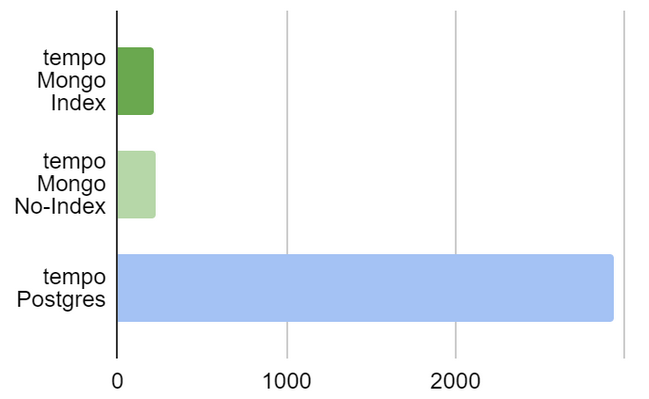
\includegraphics[height=16em]{immagini/query/query2_results1.png}
\caption{Risultato del confronto, query numero 2}
\end{center}
\end{figure}

\noindent Questa query è stata testata su database contenenti 500.000 elementi, chiedendo loro di restituirne soltanto la metà.\\
In Figura 6.4 si può vedere come, a prescindere dalla presenza dell'indice, MongoDB sia comunque più veloce di un ordine di grandezza.\\
Inoltre, grazie agli strumenti messi a disposizione da PostgreSQL, possiamo anche vedere come è stato speso il tempo all'interno di questa query (Figura 6.5).

\begin{figure}[htbp]
\begin{center}
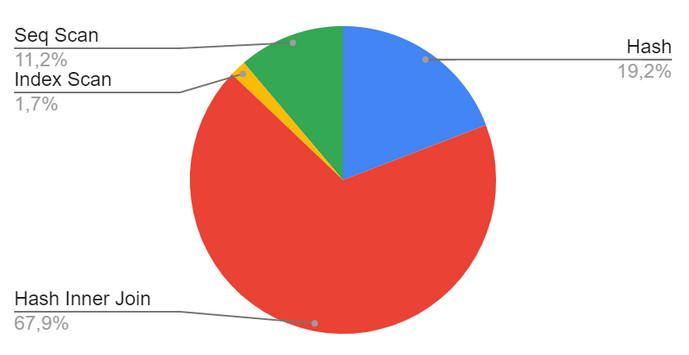
\includegraphics[height=15em]{immagini/query/query2_results2.png}
\caption{Utilizzo del tempo di esecuzione, query numero 2}
\end{center}
\end{figure}

\noindent Quasi il 70\% del tempo è dedicato all'operazione di \texttt{join}, di cui invece MongoDB non si deve preoccupare (in questo caso).\\
La sola operazione di Index Scan occupa PostgreSQL per circa 90 ms, un tempo che sarebbe estremamente competitivo.\\

%--------------------------------------------------------------

\subsection{Query 3}
A confermare la tesi portata con la seconda query, effettuare una ricerca su un campo non indicizzato, in cui non è richiesto alcuna operazione di \texttt{join}, produce risultati più o meno simili per entrambi i sistemi: ~240ms per MongoDB contro i ~300ms per Postgres (query esposta in Figura 6.6).\\
Anche in questo caso i test sono stati effettuati su database contenenti 500.000 elementi. Non sono riportati grafici a causa della minima differenza di prestazioni.\\

\begin{figure}[htbp]
\begin{center}
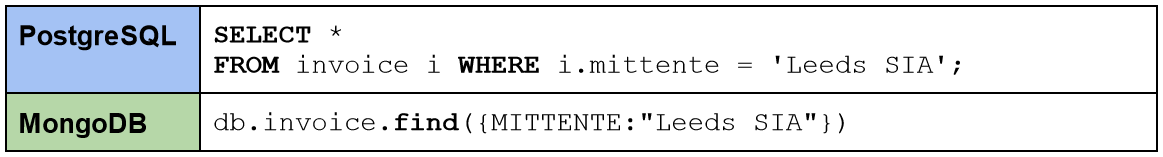
\includegraphics[height=5em]{immagini/query/query3.png}
\caption{Codice della query numero 3, scritto in entrambi i linguaggi}
\end{center}
\end{figure}

%--------------------------------------------------------------

\subsection{Query 4}
La query esposta in Figura 6.7 risulta utile per evidenziare un'altra differenza importante tra i due database, dovuta al diverso metodo di archiviazione dei dati (documenti \texttt{JSON} o tabelle).\\

\begin{figure}[htbp]
\begin{center}
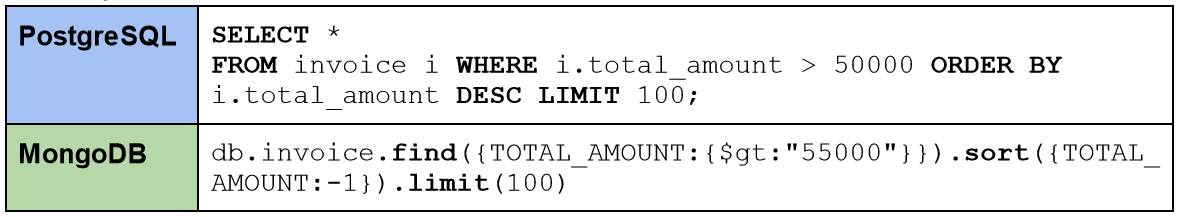
\includegraphics[height=7em]{immagini/query/query4.png}
\caption{Codice della query numero 4, scritto in entrambi i linguaggi}
\end{center}
\end{figure}

\noindent In questo caso vengono testati entrambi i database con 100.000 elementi inseriti.\\
Si vogliono trovare i documenti con data di invio più recente. Dover accedere al contenuto dei campi sembrerebbe essere un lavoro più dispendioso quando si tratta di un campo di un documento, piuttosto che un campo di una tabella. Nel grafico riportato in Figura 6.8 si nota infatti che il risultato ottenuto conferma questa tesi.\\

\begin{figure}[htbp]
\begin{center}
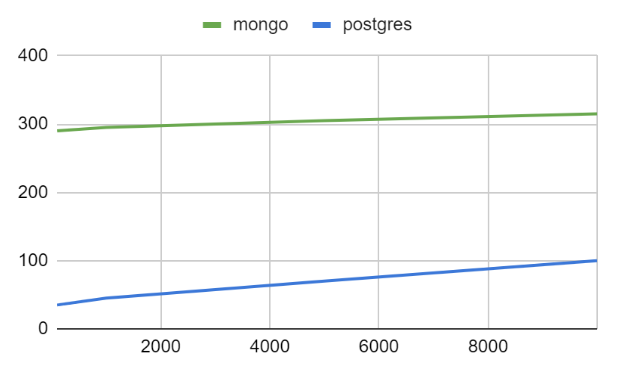
\includegraphics[height=15em]{immagini/query/query4_results.png}
\caption{Risultato del confronto, query numero 4}
\end{center}
\end{figure}

%--------------------------------------------------------------

\subsection{Query 5}
Viene testata ora una query più complessa, utilizzata per effettuare l'update di determinati campi all'interno del database. Nello specifico, si vogliono simulare l'update della causale della fattura, con delle condizioni che comprendono dati dell'operation ad essa collegata.\\

\begin{figure}[htbp]
\begin{center}
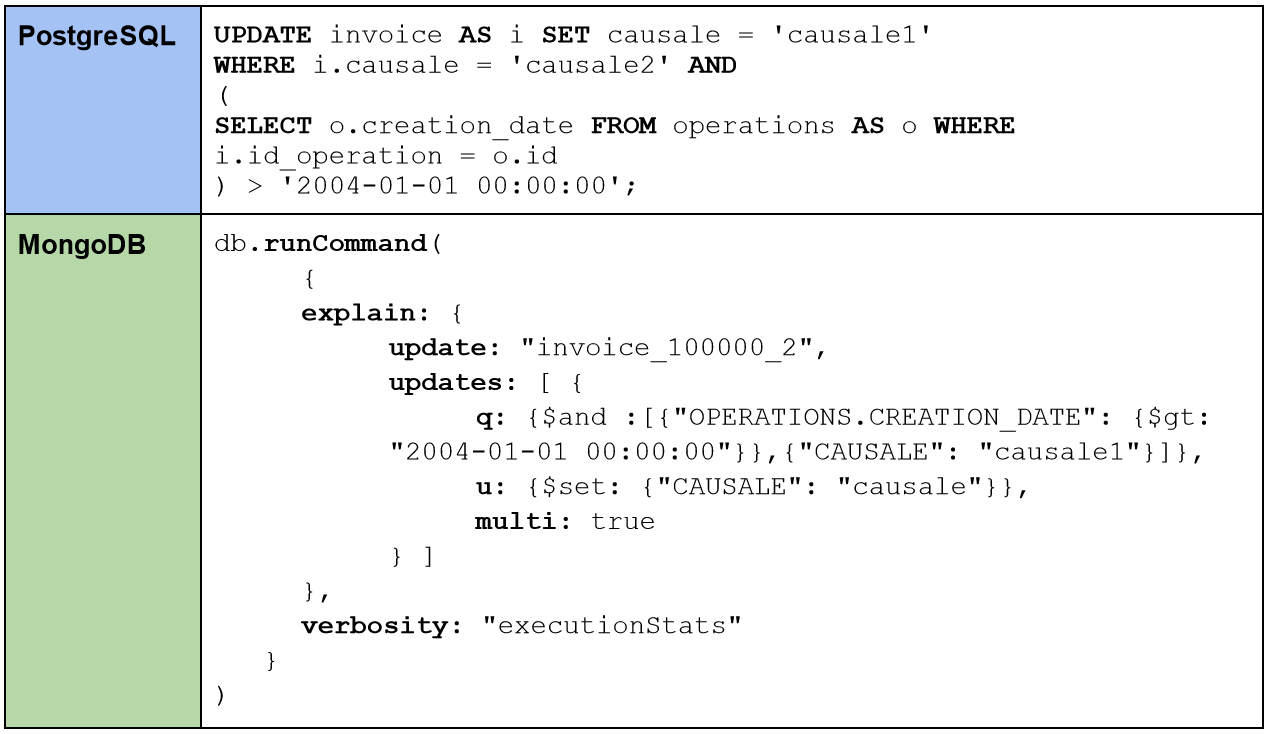
\includegraphics[height=20em]{immagini/query/query5.png}
\caption{Codice della query numero 5, scritto in entrambi i linguaggi}
\end{center}
\end{figure}

\noindent Per eseguire questa query in MongoDB, la concatenazione dei metodi è più complessa, come si può notare dalla Figura 6.9 che riporta il codice.\\
Purtroppo Compass mette a disposizione l'interfaccia explain solo per il metodo \texttt{find()}. Come detto in precedenza dobbiamo quindi passare tramite \textit{mongosh}, il terminale di MongoDB su cui si possono eseguire tutti i comandi nella sua sintassi specifica.\\
Inoltre, il sistema utilizzato precedentemente (ovvero concatenare il metodo \texttt{explain()} a fine query) non è disponibile per l'operazione di update, e bisogna quindi usare una sintassi più completa che prevede l'uso del metodo \texttt{runCommand()}, visibile in Figura 6.9.\\

\noindent Il dato importante che traspare è la differenza nei tempi di esecuzione, che anche in questo caso favoriscono MongoDB, aggirandosi intorno ai 105 ms. Per postgres abbiamo tempi all'incirca doppi.\\

%--------------------------------------------------------------

\subsection{Query 6}
La sesta query, esposta in Figura 6.10, è simile alla precedente. In questo caso tuttavia l'aggiornamento viene fatto sulla tabella \texttt{OPERATIONS}, e la condizione risiede in tabella \texttt{INVOICE}.\\

\begin{figure}[htbp]
\begin{center}
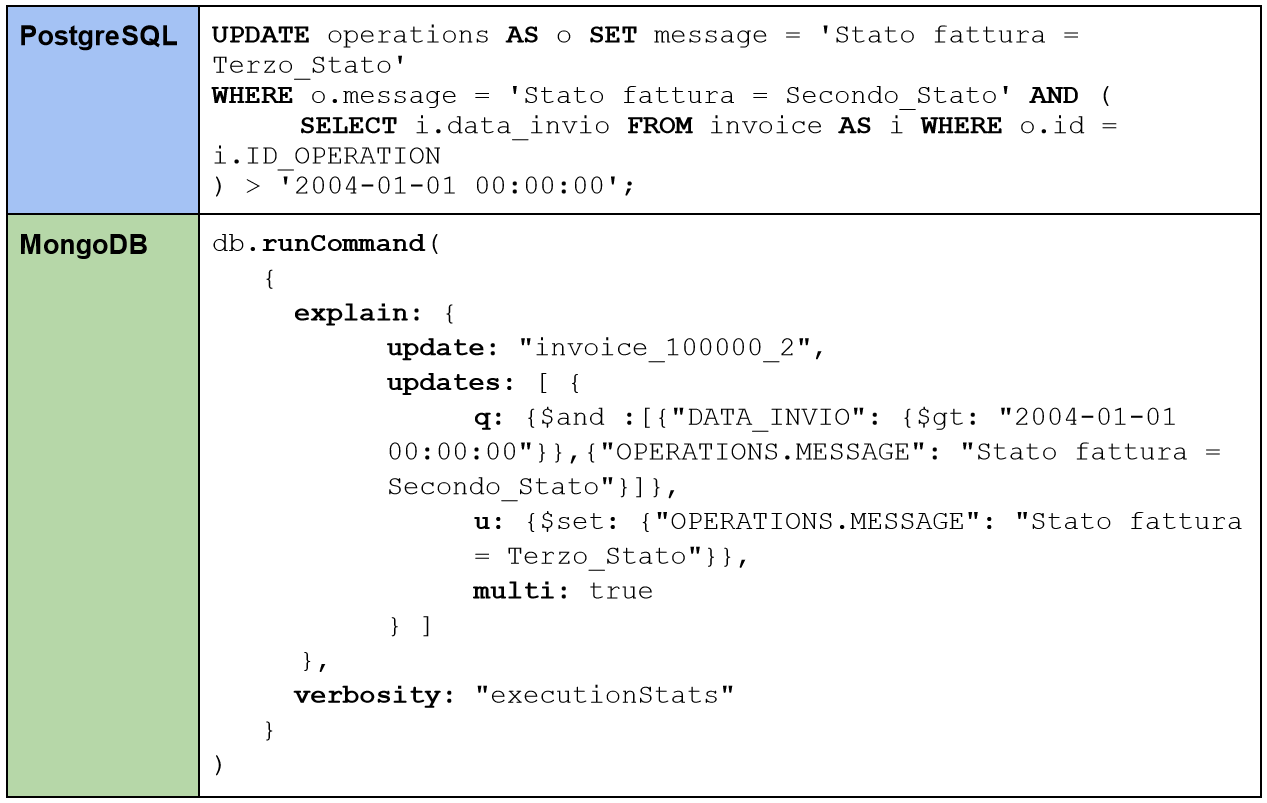
\includegraphics[height=22em]{immagini/query/query6.png}
\caption{Codice della query numero 6, scritto in entrambi i linguaggi}
\end{center}
\end{figure}

\noindent La query su PostgreSQL impiega dai 2 ai 5 minuti per essere portata a termine su un database contenente 100.000 elementi.\\
Possiamo notare come quasi tutto questo tempo sia utilizzato per effettuare uno scan della tabella \texttt{OPERATIONS}, che viene poi aggiornata.\\

% INSERIRE TABELLA AD-HOC AL POSTO DELL'IMMAGINE BRUTTA
\begin{comment}
\begin{figure}[htbp]
\begin{center}
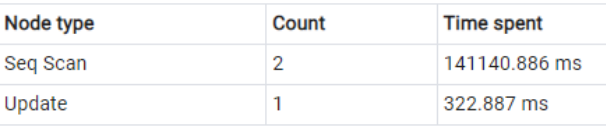
\includegraphics[height=5em]{immagini/query/query6_results.png}
\caption{Suddivisione dei tempi di esecuzione per la query numero 6 in PostgreSQL}
\end{center}
\end{figure}
\end{comment}

\noindent MongoDB impiega soltanto 65 millisecondi per effettuare tutte le operazioni.\\
Ripetendo la query su database più ampi il risultato non cambia. Per 250.000 elementi PostgreSQL impiega più di trenta minuti, MongoDB si mantiene sotto i 200 millisecondi. Il tempo raddoppia quando all'interno del database sono contenuti 500.000 elementi. Per questa quantità di dati, PostgreSQL non restituisce un risultato in tempi utili.\\

%--------------------------------------------------------------

\subsection{Query 7}
La query riportata in Figura 5.11 rappresenta un altro caso d'uso importante.

\begin{figure}[htbp]
\begin{center}
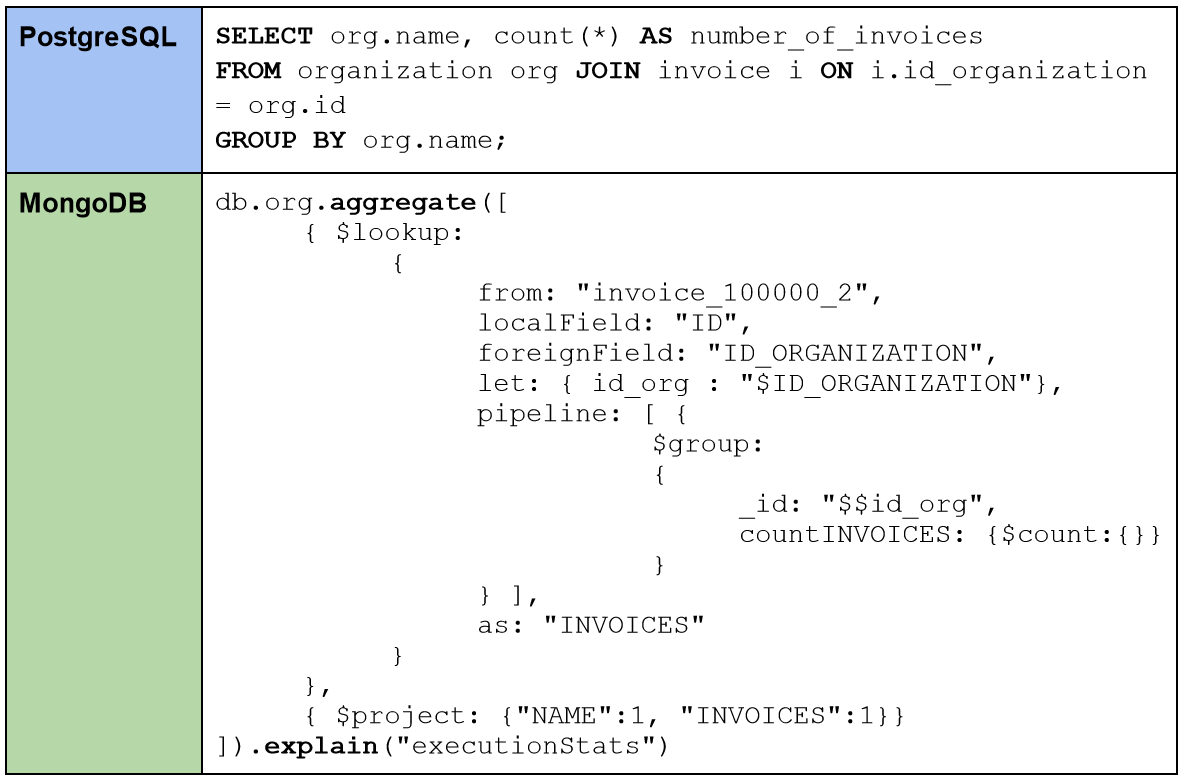
\includegraphics[height=22em]{immagini/query/query7.png}
\caption{Codice della query numero 7, scritto in entrambi i linguaggi}
\end{center}
\end{figure}

\noindent Come già menzionato, MongoDB è sì un database NoSQL, ma tecnicamente è considerabile anche ``relazionale'', perchè consente di effettuare operazioni di \textit{lookup} tra \textit{collection} diverse per unire informazioni altrimenti separate. Questa, tuttavia, non è sicuramente la feature di punta di un database documentale, e si traduce quindi in un'operazione piuttosto lenta rispetto ad altre operazioni per cui un un database di questo tipo è stato espressamente studiato.\\

\noindent Tutto questo è dimostrato dai dati statistici raccolti durante l'esecuzione delle query e riportati in Figura 5.12.\\
Per PostgreSQL si tratta di una join piuttosto semplice, accoppiata ad un raggruppamento. Il tempo di esecuzione si aggira intorno ai 65 ms se le tabelle \texttt{INVOICE} e \texttt{ORGANIZATION} contengono 100.000 elementi ciascuna.\\
MongoDB impiega tra i 5 e i 6 secondi per la stessa operazione, con la stessa quantità di dati.

\begin{figure}[htbp]
\begin{center}
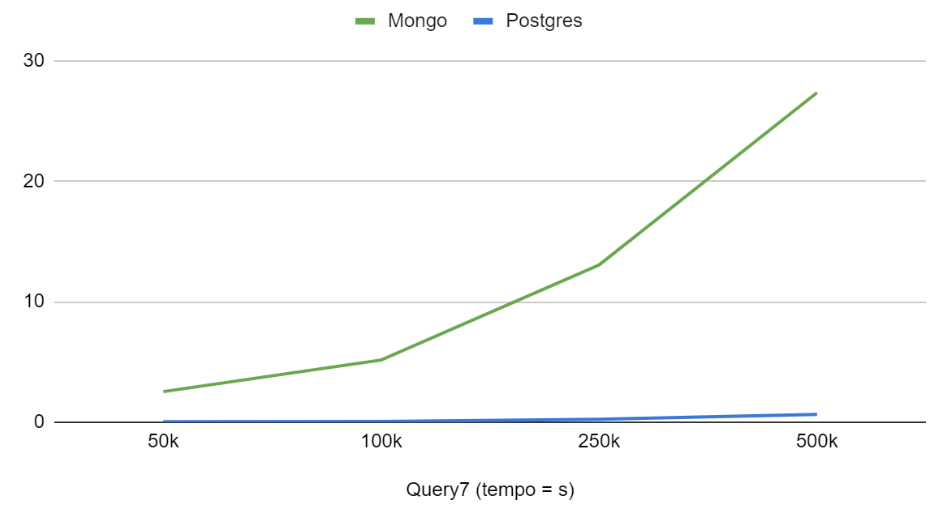
\includegraphics[height=15em]{immagini/query/query7_results.png}
\caption{Risultato del confronto, query numero 7}
\end{center}
\end{figure}

\noindent Con questa query si conclude la fase di confronto diretto tra i tempi di esecuzione delle operazioni sui due database. Vale la pena di evidenziare un fattore che sicuramente salta all'occhio leggendo le precedenti pagine: la complessità del linguaggio utilizzato per le query di MongoDB non è trascurabile e rispetto all'immediatezza di \gls{SQL}\ped{G} risulta piuttosto impegnativo da imparare, utilizzare e comprendere.

%**************************************************************
\section{Inserimento della fattura integrale}
\label{sec:fattura-integrale}
Uno dei casi d'uso di interesse per l'analisi condotta su InvoiceChannel è quello che riguarda il salvataggio delle fatture.\\
Sebbene parte dei dati che le compongono sia salvata nella tabella invoice, per velocizzare l'accesso alle informazioni più importanti la fattura viene anche salvata per intero in formato \texttt{XML}.\\

\noindent Questo ovviamente non può essere fatto all'interno del database, principalmente perchè salvare una così grande quantità di dati all'interno di un unico campo non è desiderabile.\\
All'estremo opposto c'è la possibilità di elaborare il contenuto del file per scomporlo in campi salvabili e indicizzabili, potendo così ricomporre la fattura quando necessario. Anche questa soluzione presenta delle criticità, perchè effettuare operazioni di questo tipo su ogni fattura introdotta nel sistema creerebbe probabilmente un collo di bottiglia, e anche ricomporla quando necessario potrebbe rivelarsi costoso o non pratico.\\

\noindent La soluzione, come spesso succede, sta nel mezzo, e se ne trova un esempio all'interno dell'architettura di MongoDB, come di seguito riportato.\\
Come è stato visto, MongoDB salva i propri documenti in formato \texttt{JSON}, introducendo degli ``effetti collaterali'' che tornano utili al nostro caso d'uso.\\
L'idea è di convertire le fatture da \texttt{XML} a \texttt{JSON} per poi salvarle integralmente all'interno di una collection apposita.\\
In questo modo la fattura sarebbe sempre a disposizione per intero all'interno del database, come se fosse stato inserito il file \texttt{XML} in un campo di tabella. Allo stesso tempo sarebbe facile effettuare ricerche sui ``campi'' che compongono la fattura, per natura stessa dei file \texttt{JSON}, senza dover fare alcuna operazione di scomposizione e ricostruzione del file, se non per l'iniziale traduzione da un formato all'altro.\\

\noindent Tale trasformazione è bidirezionale, quindi così come si è passati dall'\texttt{XML} al \texttt{JSON} si può fare il contrario senza alcuna perdita di dati. Questo è importante perchè a livello legale \texttt{XML} rimane il formato ufficiale per le fatture elettroniche, quindi in caso di necessità si può ricostruire l'originale.\\

\noindent Tutto questo ovviamente ha un costo, e sta a chi crea un sistema di questo tipo il compito di soppesare pro e contro. MongoDB supporta l'inserimento di file \texttt{BSON} fino a 16 MB e una fattura tradotta in formato \texttt{JSON} occupa circa 5 KB, quindi sebbene appaia come un file ``grande'' all'occhio umano, si tratta di una dimensione bel al di sotto dei limiti strutturali del database. Le prestazioni non sarebbero intaccate da questo tipo di soluzione, anche quando si considera l'archiviazione di centinaia di migliaia di fatture, specialmente se si fa uso di indici.\\
Anche il costo della traduzione da \texttt{XML} a \texttt{JSON} va sicuramente rendicontato, ma dai test condotti non sembra avere un grosso impatto. Utilizzando uno strumento esterno basato su \gls{npm}\ped{G} (come \textit{datamaker}) è possibile automatizzare questo processo ad un bassissimo costo computazionale.\\

% Inserire conclusioni sulla fattura integrale
